\section{RASCUNHO}

    % FIXME: REMOVER ESSE CAPITULO NO FINAL
    
\begin{verbatim}
> artigo mateus: sessao 4 (38)
> usar como referencia para escrever as restricoes de dwell time
> usando a restricao da 3.4, Su = -L, Bu = -c
\end{verbatim}

==============================================

TL;DR

\begin{figure}[h]
    \centering
    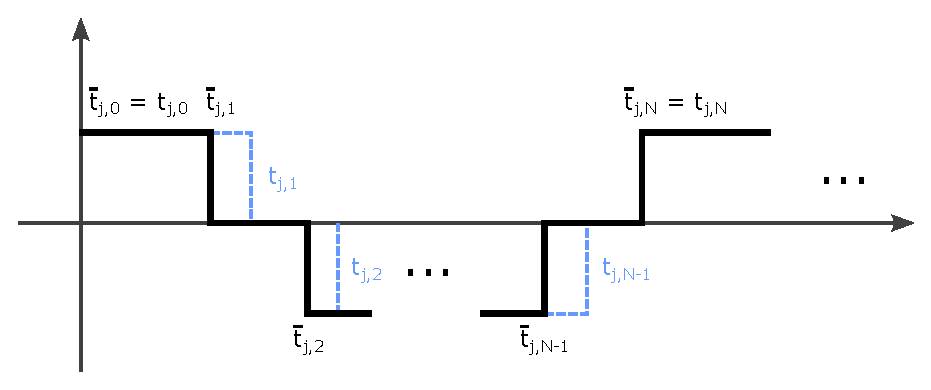
\includegraphics[]{figures/cap4/desenho_cap4.eps}
    \caption{Instantes de chaveamento}\label{bla_rascunho}
\end{figure}

a restricao que queremos impor �:

\noindent
\begin{equation}
    (t_i - t_{i - 1}) \ge \Delta t_{i,min}\;, \quad i = 1,2,\dotso,N
\end{equation}

como

\noindent
\begin{equation}
    \Delta \bar{t}_i = \bar{t}_i - \bar{t}_{i-1}
\end{equation}

ent�o podemos escrever a restricao da seguinte maneira

\noindent
\begin{align}
        \delta t_1 &\ge - \Delta \bar{t}_1 + \Delta t_{1,min} \\
        \delta t_i - \delta t_{i-1} &\ge - \Delta \bar{t}_i + \Delta t_{i,min}\;, \quad i = 1,2,\dotso,N \\
        \delta t_{N-1} &\ge - \Delta \bar{t}_N + \Delta t_{N,min}
\end{align}

que pode ser representado na forma matricial como

\begin{equation}
    \mathbf{L} = 
    \left[
        \begin{matrix}
             1 & 0 & 0 & \dotsi &  0 &  0 \\
            -1 & 1 & 0 & \dotsi &  0 &  0 \\
            \vdots & \vdots & \vdots & \ddots & \vdots & \vdots \\
             0 & 0 & 0 & \dotsi & -1 &  1 \\
             0 & 0 & 0 & \dotsi &  0 & -1 \\
        \end{matrix}
    \right]
\end{equation}

\begin{equation}
    c = 
    \left[
        \begin{matrix}
            -\Delta t_{r_1} + -\Delta t_{r_{1, min}} \\
            -\Delta t_{r_2} + -\Delta t_{r_{2, min}} \\
            \vdots \\
            -\Delta t_{r_{N-1}} + -\Delta t_{r_{{N-1}, min}} \\
            -\Delta t_{r_N} + -\Delta t_{r_{N, min}} \\
        \end{matrix}
    \right]
\end{equation}

==============================================

4 Predictive Control Formulation

The problem addressed herein consists in determining suitable perturbations in the switching times of the input signal to drive the state deviation
e[k] to zero asymptotically. As a result, the state x[k] will be driven to the target point $x_r (t_0) = x_r (t_N)$.

For this purpose, the discrete-time model (28) derived in the previous section is employed within a predictive control framework. 
The cost function to be minimized at the beginning of the kth oscillation cycle is chosen as

\begin{equation}
    J = \norma{\hat{e} \Big[k = N_p[k] \Big]}{P_f}
    + \sum_{j=1}^{N_p} \norma{\hat{e} \Big[ k + j|k\Big]}{Q}
    + \norma{\hat{\delta_t} \Big[ k + j - 1 | k\Big]}{R}
\end{equation}

where $Q = Q_T \in \mathbb{R}^{n \times n}$, $R = R_T \in \mathbb{R}^{(N-1) \times (N-1)}$, $P_f = P_f^T \in \mathbb{R}^{n \times n}$ are positive-definite 
weight matrices. Following standard predictive control notation, the hat and $[\dot|k]$ symbols are used to indicate that 
$\hat{\delta t}[k|k], \hat{\delta t}[k+1|k], \hat{\delta t}[k+N_p|k]$ is a sequence of 
manipulated vectors which are to be optimized over a prediction horizon spanning $N_p$ 
oscillation cycles. The relation between these manipulated vectors and the predicted state deviations is given by.

\begin{equation}
    \begin{gathered}
        \hat{e}[k|k] = e[k] \\
        \hat{e}[k + j|k] = \Phi \hat{e}[k + j -1 |k] + \Gamma \hat{\delta} t [k + j - 1 |k], \\
        j = 1,2,\dots, N_p
    \end{gathered}
\end{equation}

In order to enforce (8) - (10) at each oscillation cycle, the following constraints will be imposed:

\begin{equation}
    \mathbf{L} \hat{\delta t} [k + j - 1|k] \ge c, j = 1,2, \dots, N_p
\end{equation}

with $\mathbf{L} \in \mathbb{R}^{N \times (N-1)}$ and $c \in \mathbb{R}^{N \times (N-1)}$ and $c \in \mathbb{R}^{N}$ given by 

\begin{equation}
    \mathbf{L} = 
    \left[
        \begin{matrix}
             1 & 0 & 0 & \dotsi &  0 &  0 \\
            -1 & 1 & 0 & \dotsi &  0 &  0 \\
            \vdots & \vdots & \vdots & \ddots & \vdots & \vdots \\
             0 & 0 & 0 & \dotsi & -1 &  1 \\
             0 & 0 & 0 & \dotsi &  0 & -1 \\
        \end{matrix}
    \right]
\end{equation}

\begin{equation}
    c = 
    \left[
        \begin{matrix}
            -\Delta t_{r_1} + -\Delta t_{r_{1, min}} \\
            -\Delta t_{r_2} + -\Delta t_{r_{2, min}} \\
            \vdots \\
            -\Delta t_{r_{N-1}} + -\Delta t_{r_{{N-1}, min}} \\
            -\Delta t_{r_N} + -\Delta t_{r_{N, min}} \\
        \end{matrix}
    \right]
\end{equation}

Moreover, nominal stability for the closed-loop system can be obtained by imposing a constraint on the form

\begin{equation}
    \hat{e} [k + N_p | k] \in \mathbb{E}_f
\end{equation}